\documentclass[tikz, border=0pt]{standalone}
\usepackage{graphicx}
\usepackage{xcolor}
\usetikzlibrary{patterns,calc}

\begin{document}
	\begin{tikzpicture}
		% Nodo principal con la imagen (aquí defines el tamaño)
		\node[inner sep=0] (fig_2d) {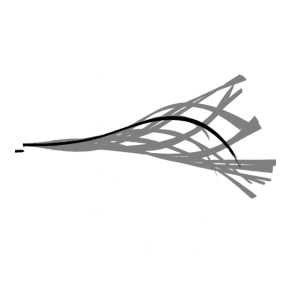
\includegraphics[width=10cm]{2D_flag_snapshots}};
		
		% Entorno scope que usa las coordenadas relativas al nodo de la imagen
		\begin{scope}[shift={(fig_2d.south west)}, x={(fig_2d.south east)}, y={(fig_2d.north west)}]
			% Todas las coordenadas ahora son relativas (0-1 en x, 0-1 en y)
			
			% Rectángulo blanco (ejemplo: 10% ancho, 10% alto desde esquina SW)
			\fill[white] (0,0) rectangle (0.1,0.1);
			
			% Línea naranja (posicionada en x=0%, y=20% del alto)
			\draw[line width=0.02, orange] (0,0.2) -- (0.1,0.2);
			
			% Flechas de viento (usando coordenadas relativas)
			\foreach \y in {0.05,0.10,...,0.30}{
				\draw[->,thick] (0.1,\y) -- (0.2,\y);
			}
			
			% Curva compleja (coordenadas relativas)
			\draw[thick] (0.1,0.15) .. controls (0.15,0.15) and (0.2,0.25) .. (0.3,0.4);
		\end{scope}
	\end{tikzpicture}
\end{document}z